\chapter{Design and Requirements}
\label{chap:figtab}
\label{chap}
\section{Requirements}\label{requirements}
The objective of this software is to  design a dynamic user interface and a functional database system. With regard to that, the specification is made up of necessary features and functionality that must appear on the user interface. The following are the major specification of this software:
\begin{description}
\item[$\bullet$] Data Inventory
\item[$\bullet$] Searching Inventory (SI)
\item[$\bullet$] Make Reservations
\item[$\bullet$] Cancel Reservations
\item[$\bullet$] Add and Update Data
\end{description}
\subsection{Data Inventory}
The user interface is able to list the inventory of data stored in the database in different categories. It is one of the features of the user interface because it presents the content of the database. Data inventory is required to retrieve information from the database and requested by users on the interface. For example, when users need to see the list of test machines in the system, this feature is responsible for providing the information already on the web interface. We have the ability to access this inventory faster by adding some functionality in the interface. Example is the ability to sort the inventory chronologically or by data sequence. 
\subsection{Searching Inventory} \label{searchinventory}
As there are lots of different data listed in the inventory, it is necessary to have a function that allows users to search for information in the inventory. Searching the inventory helps the users to get specific data by typing in queries such as dates, times, NFS root, PXE and memory sizes of a particular machine or reservation. Users can search for a particular reservation by specifying a range of data they want to see, and this will present the lists of reservations made within that date and so on. Another example of searching inventory is where users can search for available machines, and therefore allowing the user to know which machine is free for reservation.
\subsection{Make Reservation}\label{makereserve}
Another requirement of this software is the ability to make reservations: users are able to choose a machine from the inventory and reserve it for a fixed date and time. This requirement on the high level is meant to allow user to reserve a machine for running a particular task on that machine without interruption. When a reservation made is expired, the machine that was reserved becomes free for other users. 
\subsection{Add and Update Data} \label{addmachines}
As new machines are added to the cluster, the Add-data functionality allows users to add details of those machines to the database and update the inventory. Likewise, when the user want to change a certain properties of the machines such as, memory size or disk, the Update-data functionality helps to validate  this changes in the database.

\section{Design} \label{Designstructure}
The design structure comprises the various  segments and element of the user interface (front end) combined with the database (back end). In this design some of the components such as the database structure has been worked on by others, so I added more functionality during the implementation that contributed to the requirements. I worked on  methods that helps in searching for unreserved machines, sorting data, updating data and filtering inventory, making reservations and creating new Disks and NICs.  Figure~\ref{fig:Design} describes the main structure of the design in terms of operation.
\begin{figure}[h]
  \includegraphics[width=\linewidth]{Design.eps}
  \caption{The Design}
  \label{fig:Design}
\end{figure}
\pagebreak
We augmented the web interface that provides  flexible and dynamic access to the system with interactive functionality. This web page contains inputs and output features. The reason for choosing a web page instead of other options is to provide online dynamic and simultaneous  access to the system rather than performing manual command prompts. Another reason is to have a functional user interface that present the activities of the Clowder. The web server is responsible for serving the web page with all the resources requested by the users, and it serves as a channel between the user and the database. The database stores data from the web page and also retrieves data on the web page via the server. As the user log on to web page the server will pass this information to the database which is controlled by the main program. 

\subsection{User Interface}
The web interface represents the user interface (UI) where users get access to the system. It is part of the design that represents the front end of the software.The web interface elements controls the basic functionality for data input and out put. It represent each feature as mentioned in the specification. This web interface structure is designed using  HTML template for the front end and Go programming language for the back end. 
The web interface contains all the necessary elements required to have dynamic and flexible access to the system. These elements include Forms and Input controls.
\subsection*{Forms}
Forms are one  of the elements that provides the ability to input data to the database. The data is submitted through a HTTP POST request \cite{WinNT}. The post forms are used for submitting data such as machines and reservations details. The form is designed with elements which includes id and name attributes for identifying data, text fields for collecting data, select menus for selecting data options and submit button for submitting the data. When data is submitted with HTTP form, the Go HTTP framework in the web server call a registered Go function handler to process and parse this data to the database.  After the data (example: a database query) is processed, the Go program generates an HTML page (such as machines inventory), which the server returns to the web interface. In this system design, the forms are used for creating new machines, disks, NICs and making reservation. 
\subsection*{Input Controls}
The input control in this web interface provides the necessary components that supports the functionality of the software. There are numerous HTML input control, but we have chosen a few that satisfy our specifications. These input controls include text fields, buttons, date fields, drop down list and list box. They are used for both input and output functions like listing the inventory, inserting texts, to update data, to send queries, viewing selection options and searching inventory. These controls are designed with HTML tags and HTML template.
\subsection{Web Server}
The server is responsible for parsing all requests from the web interface. When a request is made on the web interface (for instance querying available machines), the server calls the a function to handle this request by providing the necessary resources. And interchanging communication between the user interface and the database system for executions and requests. 
\begin{figure}[h!]
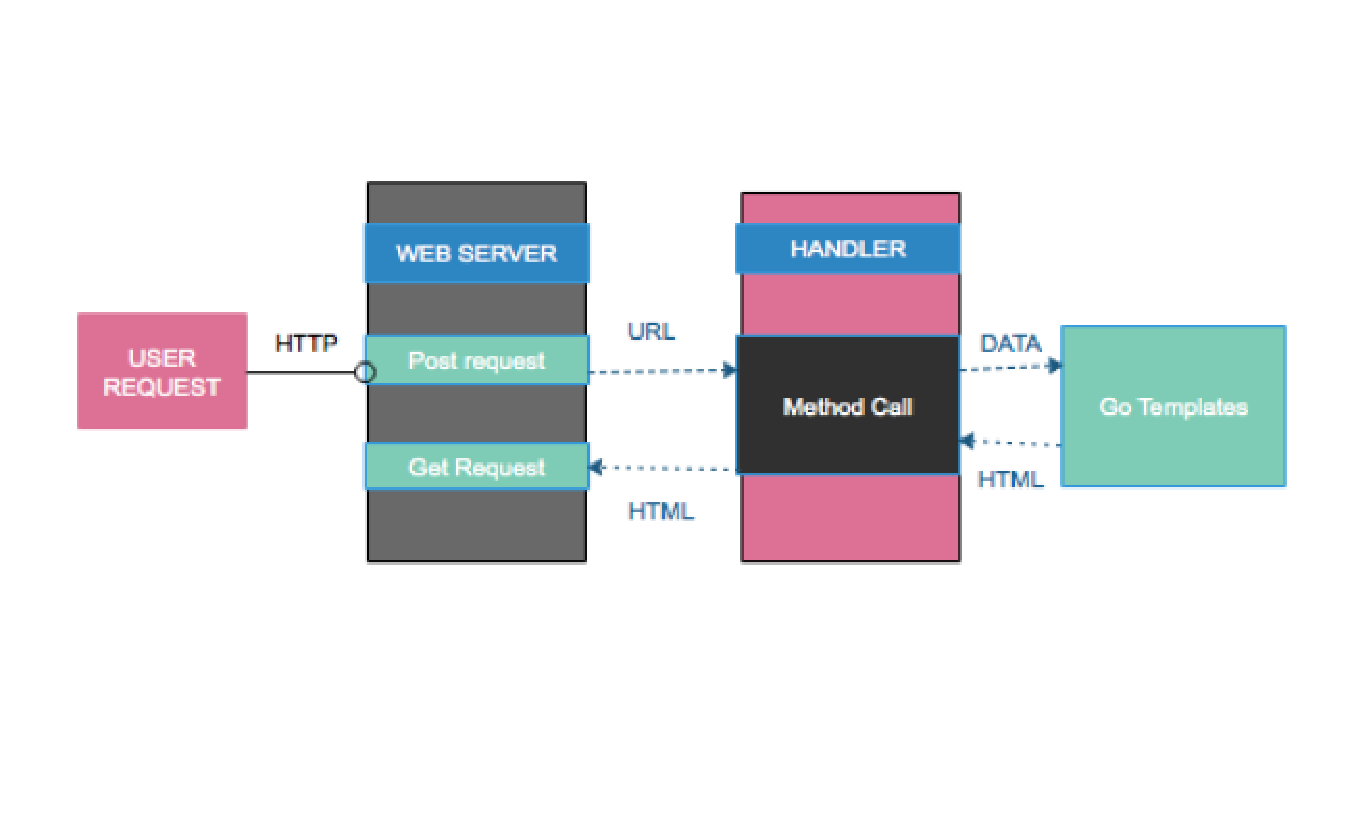
\includegraphics[width = \linewidth]{server1.eps}
\label{fig:Description of Server Activity} 
\caption{Server Activity Description}
\end{figure}

\pagebreak
\subsection{Database}
The database is another major component of this system, because it is provides storage and resource for the system. The data includes reservation records, machine details, disks, and NICs (network interface card) information. The database is designed with SQL model using Go programming language as the back end tech. SQL was used here as prototype because it is fast and easy to set up. We created a functional database system that address the specification of the software. 
The database scheme contains tables of machines, user record, reservation, NICs and disks.  One of the functions of the software is the ability to make reservations. \autoref{Databaseschema} shows a typical model of the database design.
\begin{figure}[h!]
\includegraphics[width = \linewidth]{database.eps}
\caption{Database design}
\label{Databaseschema} 
\end{figure}
\subsection{Data Flow}
The data flows from the user interface via the web server to the database. We used Go HTTP handlers to process data received from the HTML form to be stored in the database. The server initiates each method (function) when the HTTP handler sends a request. For example, when users search for list of information such as machine details, the request is sent through the server as a query, and the appropriate Go function is called to fetch the data from the designated database. Go HTTP handler uses a Request functon to call the server and  ResponseWriter to respond to the HTML request \cite{Gohttp}. The server uses ListenAndServe method to listen to incoming request and to call the requested method to handle the request. This process controls the sequence of data flow in the system. It controls data input, handling and output. This protocol helps the dynamic functionality on the user interface to perform in the system and also provides automatic command rather than manual query routine performed on command line. \autoref{sort} shows example of  handler function and \autoref{callsort} shows the registered function in the server.
\lstset{basicstyle=\footnotesize\ttfamily,breaklines=true}
\lstset{framextopmargin=50pt,frame=bottomline}
\begin{lstlisting}[caption=Sort Memory function in the handler, label=sort]
func (s Server) sortmPage(w http.ResponseWriter, r *http.Request) {
	s.logRequest(r)
	tname := "machines.html"
	t, err := getTemplate(tname)
	if err != nil {
		s.Error(err)
		templateError(w, tname, err)
		return
	}
	sortmemory,err := s.db.Sort_Memory()
		if err != nil {
		s.db.Error(err)
		renderError(w, "Error sorting",
			fmt.Sprintf("Unable to sort machines: ",
				err))
		return
	}
	t.Execute(w, sortmemory)
}
\end{lstlisting}

\lstset{basicstyle=\footnotesize\ttfamily,breaklines=true}
\lstset{framextopmargin=50pt,frame=bottomline}
\begin{lstlisting}[caption=Calling Sort Memory function, label=callsort]
http.HandleFunc("/machines/Sort_Memory/", server.sortmPage)
\end{lstlisting}

